%\documentclass[handout]{beamer}
\documentclass[usenames,dvipsnames]{beamer}
\usepackage{amsmath}
\usepackage{stdpresent}
%\usepackage[margin=1in]{geometry}
\usepackage{tikz}
\usepackage{booktabs}
\usepackage{subcaption}
\captionsetup{compatibility=false}
\usepackage{tikz}
\usetikzlibrary{intersections,positioning}
\usetikzlibrary{matrix, calc}
\newcommand*{\hnode}[1]{\node[outer sep=0pt,anchor=base] (#1) {#1};} 
\usepackage[absolute,overlay]{textpos}
\usetikzlibrary{bayesnet}
\usepackage{tcolorbox}
\usepackage[tikz]{bclogo}
\usepackage{textcomp}
\usepackage{vimacros}
\usepackage{physics}
\usepackage[round]{natbib}

\beamertemplatenavigationsymbolsempty
%\hypersetup{breaklinks=true, colorlinks=true, linkcolor=blue, citecolor=blue, urlcolor=blue}
\newcommand{\ack}[1]{\let\thefootnote\relax\footnote{\textcolor{gray}{#1}}}

\usepackage{tikz}
\usetikzlibrary{bayesnet}

\newcommand{\SDEC}{SDEC}
\newcommand{\SENT}{SENT}


%\DeclareMathOperator*{\softmax}{softmax}

\title[DGMs in NLP]{Variational Auto-encoders}


\def\W#1#2{\rnode{#1}{#2}\hfill}

\newcommand{\pointthis}[2]{
        \tikz[remember picture,baseline]{\node[anchor=base,inner sep=0,outer sep=0]%
        (#1) {\textbf{#1}};\node[overlay,rectangle callout,%
        callout relative pointer={(0.1cm,0.5cm)},fill=yellow!90] at ($(#1.north)+(-.5cm,-1cm)$) {#2};}%
        }%

\presetkeys{bclogo}{
ombre=true,
epBord=3,
couleur = blue!15!white,
couleurBord = red,
arrondi = 0.2,
logo=\bctrombone
}{}

\author[Miguel Rios]{Miguel Rios\\University of Amsterdam}
\date{\today}

% add page num
\expandafter\def\expandafter\insertshorttitle\expandafter{%
  \insertshorttitle\hfill%
  \insertframenumber}

\begin{document}
\maketitlepage


\setcounter{framenumber}{0}

%\section{Deep generative models}


\begin{frame}{Problems}

{\bf Supervised} problems
\begin{center}\emph{``learn a distribution over \textcolor{blue}{observed} data''}\end{center}

\begin{itemize}
	\item \textcolor{black}{sentences in natural language}
	\item images, \ldots
\end{itemize}

~ \pause

{\bf Unsupervised} problems
\begin{center}\emph{``learn a distribution over \textcolor{blue}{observed} and \textcolor{red}{unobserved} data''}\end{center}
\begin{itemize}
	\item \textcolor{black}{sentences in natural language + parse trees}
	\item images + bounding boxes, \ldots
\end{itemize}
\end{frame}


\begin{frame}{Supervised problems}

\small

We have data $x^{(1)}, \ldots, x^{(N)}$ e.g.  \\
\begin{itemize}
	\item sentences, images, ...
\end{itemize}
generated by some {\bf unknown} procedure

\pause

which we assume can be captured by a probabilistic model

\pause

\begin{itemize}
	\item with {\bf known} probability (mass/density) function e.g.
	\begin{align*}
    \underbrace{X \sim \Cat(\alert{\pi_1}, \alert{\ldots}, \alert{\pi_K})}_{\text{e.g. nationality}} & & \text{or} & & \underbrace{X \sim \mathcal N(\alert\mu, \alert\sigma^2)}_{\text{e.g. height}}
    \end{align*}    
\end{itemize}
\pause
\alert{estimate parameters} that assign maximum likelihood to observations

%\pause
%e.g. $\pdv{\pi_j} \sum_{i=1}^N \log \Cat(X=x^{(i)}|\pi_1^K) $\\
%e.g. $\pdv{\mu} \sum_{i=1}^N \log  \mathcal N(X=x^{(i)}|\mu, \sigma^2)$

\end{frame}

\begin{frame}{Multiple problems, same language}



\begin{small}

\begin{columns}
\begin{column}{0.3\textwidth}
\scalebox{0.8}{
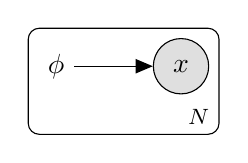
\begin{tikzpicture}
\node[obs] (x) {$ x $};
\node[left=of x] (phi) {$ \phi $};

\edge{phi}{x};

\plate {data} {(x)(phi)} {$ N $};
\end{tikzpicture}
}
\end{column}
\begin{column}{0.6\textwidth}
\alert{(Conditional) Density estimation}
\end{column}

\end{columns}

\begin{tabular}{p{2cm} p{4cm} p{4cm}}
 & Side information ($\phi$) & Observation ($x$) \\ \cline{2-3}
Parsing &   \textcolor{black}{a sentence} & \textcolor{blue}{parse tree} \\
&&\\
Translation &  \textcolor{black}{a sentence in French} & \textcolor{blue}{translation in English} \\
&&\\
Captioning &  \textcolor{black}{an image} & \textcolor{blue}{caption in English} \\
&&\\
Entailment  & \textcolor{black}{a text and hypothesis} & \textcolor{blue}{entailment relation}
\end{tabular}
\end{small}

\end{frame}

\begin{frame}{Where does deep learning kick in?}

Let $\phi$ be all side information available\\
~ e.g. deterministic \emph{inputs/features}

~ \pause

Have neural networks predict parameters of our probabilistic model
	\begin{align*}
    X|\phi \sim \Cat(\pi_{\alert \theta}(\phi)) & & \text{or} & & X|\phi \sim \mathcal N(\mu_{\alert \theta}(\phi), \sigma_{\alert \theta}(\phi)^2)
    \end{align*} \pause
~ and proceed to \alert{estimate parameters} $\theta$ of the NNs %via MLE % that assign maximum likelihood to observations

 





\end{frame}


\begin{comment}
\begin{frame}{Task-driven feature extraction}

Often our side information $\phi$ is itself some high dimensional data
\begin{itemize}
	\item $\phi$ is a sentence and $x$ a tree
	\item $\phi$ is the source sentence and $x$ is the target
	\item $\phi$ is an image and $x$ is a caption
\end{itemize}
and part of the job of the NNs that parametrise our models is to also \alert{deterministically} encode that input in a low-dimensional space

\end{frame}
\end{comment}


\begin{frame}{NN as efficient parametrisation}

From the statistical point of view NNs do not generate data\\
\begin{itemize}
	\item \alert{they parametrise distributions} that \\
	\emph{by assumption} govern data
	\item compact and efficient way to \alert{map from complex side information to parameter space}
\end{itemize}

\vspace{10pt}

\pause
Prediction is done by a decision rule outside the statistical model
\begin{itemize}
	\item e.g. beam search
\end{itemize}

\end{frame}

\begin{frame}{Maximum likelihood estimation}

Let $p(x|\theta)$ be the probability of an observation $x$\\
~and $\theta$ refer to all of its parameters \\
~e.g. parameters of NNs involved

~ \pause

Given a dataset $x^{(1)}, \ldots, x^{(N)}$ of i.i.d. observations, the likelihood function 
\begin{equation*}
\begin{aligned}
\mathcal L(\theta|x^{(1:N)}) &= \log \prod_{s=1}^N p(x^{(s)}|\theta) \\ \pause
 &= \sum_{s=1}^N \log p(x^{(s)}|\theta)
\end{aligned}
\end{equation*} \pause
quantifies the fitness of our model to data

\end{frame}

\begin{frame}{MLE via gradient-based optimisation}

If assessing the log-likelihood is {\bf differentiable} and assessing it is {\bf tractable}, then backpropagation can give us the gradient
\begin{equation*}
\begin{aligned}
\grad_\theta \mathcal L(\theta|x^{(1:N)}) &= \grad_\theta \sum_{s=1}^N \log p(x^{(s)}|\theta) \\ \pause
 &=  \sum_{s=1}^N \grad_\theta \log p(x^{(s)}|\theta)
\end{aligned}
\end{equation*}  \pause

and we can update $\theta$ in the direction
\begin{equation*}
\gamma \grad_\theta \mathcal L(\theta|x^{(1:N)})
\end{equation*}
to attain a local optimum of the likelihood function

\end{frame}

\begin{frame}[plain]{Stochastic optimisation}

We can also use a gradient estimate 
\begin{equation*}
\begin{aligned}
\grad_\theta \mathcal L(\theta|x^{(1:N)}) &= \grad_\theta \underbrace{\mathbb E_{S\sim \mathcal U(1..N)}\left[ N \log p(x^{(S)}|\theta)\right]}_{\mathcal L(\theta|x^{(1:N)})} \\ \pause
 &=  \underbrace{\mathbb E_{S\sim \mathcal U(1..N)}\left[ N \grad_\theta  \log p(x^{(S)}|\theta)\right]}_{\text{expected gradient :)}} \\ \pause
 &\overset{\text{MC}}{\approx} \frac{1}{M} \sum_{m=1}^M N  \grad_\theta \log p(x^{(s_i)}|\theta) \\
 &S_i \sim \mathcal U(1..N)
\end{aligned}
\end{equation*}  \pause
and take steps in the direction
\begin{equation*}
\gamma \frac{N}{M} \grad_\theta \mathcal L(\theta|x^{(s_1:s_M)})
\end{equation*}
where $x^{(s_1)}, \ldots, x^{(s_M)}$ is a random mini-batch of size $M$


\end{frame}



\begin{frame}{DL in NLP recipe}


%Vast majority of papers published at ACL

%\begin{small}
%\begin{figure}
%\scalebox{0.8}{
%\begin{tikzpicture}
%\node[obs] (x) {$ x $};
%\node[left=of x] (phi) {$ \phi $};
%\factor[left=of x] {f} {below:$f_w$} {phi} {x} ; 
%%\edge{phi}{x} ;
%\plate {data} {(x)(phi)} {$ N $};
%\end{tikzpicture}
%}
%\end{figure}
%\end{small}
	Maximum likelihood estimation
	\begin{itemize}
		\item  tells you which \alert{loss} to optimise \\
		(i.e. negative log-likelihood)
	\end{itemize}
	
	\pause
	Automatic differentiation (\emph{backprop})
	\begin{itemize}
		\item chain rule of derivatives: ``give me a tractable forward pass and I will give you \alert{gradients}''
	\end{itemize}
	
	\pause
	Stochastic optimisation powered by backprop
	\begin{itemize}
		\item general purpose gradient-based optimisers
	\end{itemize}

\end{frame}


\begin{frame}{Tractability is central}

Likelihood gives us a differentiable objective to optimise for
\begin{itemize}
	\item but we need to stick with \alert{tractable} likelihood functions
\end{itemize}



%, any intractable likelihood will leave us in bad territory because
%\begin{itemize}
%	\item stochastic optimisation requires gradient estimates
%	\item which must be unbiased (forget greedy techniques)
%	\item and some estimation techniques are not differentiable (forget MC sampling)
%\end{itemize}

\end{frame}

\begin{frame}{When do we have intractable likelihood?}

{\bf Unsupervised problems} contain unobserved random variables\\ 
\begin{equation*}
p_\theta(x, z) = \overbrace{p(z)}^{\text{latent variable model}} \underbrace{p_\theta(x|z)}_{\text{observation model}}
\end{equation*}

~ \pause

thus assessing the marginal likelihood requires \alert{marginalisation of latent variables} 
\begin{equation*}
p_\theta(x) = \int p_\theta(x, z) \dd{z} = \int p(z)p_\theta(x|z) \dd{z} 
\end{equation*}


\end{frame}

\begin{frame}{Examples of latent variable models}

Discrete latent variable, continuous observation
\begin{itemize}
	\item too many forward passes
	\begin{small}
	\begin{equation*}
	p_\theta(x) = \sum_{c=1}^K \Cat(c|\pi_1, \ldots, \pi_K) \underbrace{\mathcal N(x|\mu_\theta(c), \sigma_\theta(c)^2)}_{\text{forward pass}}
	\end{equation*}
	\end{small}
\end{itemize}
	\pause
	
Continuous latent variable, discrete observation
\begin{itemize}
	\item infinitely many forward passes
	\begin{small}
	\begin{equation*}
	p_\theta(x) = \int \mathcal N(z|0, I) \underbrace{\Cat(x|\pi_\theta(z))}_{\text{forward pass}} \mathrm{d}z
	\end{equation*}
	\end{small}
\end{itemize}

\end{frame}

\begin{frame}{Deep generative models}

Joint distribution with {\bf deep observation model}
\begin{equation*}
p_\theta(x, z) = \underbrace{p(z)}_{\text{prior}} \underbrace{p_\theta(x|z)}_{\text{likelihood}}
\end{equation*}
~ {\small mapping from latent variable $z$ to $p(x|z)$ is a NN with parameters $\theta$}

~ \pause

Marginal likelihood (or evidence)
\begin{equation*}
p_\theta(x) = \int p_\theta(x, z) \dd{z} = \int p(z)p_\theta(x|z) \dd{z} 
\end{equation*}
~ \alert{intractable} in general



\end{frame}

\begin{frame}[plain]{Gradient}

Exact gradient is intractable
\begin{small}
\begin{equation*}
\begin{aligned}
\grad_\theta \log p_\theta(x) \pause &= \grad_\theta \log \underbrace{\int p_\theta(x, z) \dd{z}}_{\text{marginal}} \\ \pause
&= \underbrace{\frac{1}{\int p_\theta(x, z) \dd{z}} \int \grad_\theta p_\theta(x,z) \dd{z}}_{\text{chain rule}} \\ \pause
&= \frac{1}{p_\theta(x)} \int \underbrace{p_\theta(x,z) \grad_\theta \log p_\theta(x,z)}_{\text{log-identity for derivatives}} \dd{z} \\ \pause
&= \int \underbrace{\frac{p_\theta(x,z)}{p_\theta(x)}}_{\text{posterior}} \grad_\theta \log p_\theta(x,z) \dd{z} \\ \pause
&= \int p_\theta(z|x) \grad_\theta \log p_\theta(x,z) \dd{z} \\ \pause
&= \underbrace{\mathbb E_{p_\theta(z|x)} \left[ \grad_\theta \log p_\theta(x,Z) \right]}_{\text{expected gradient :)}}
\end{aligned}
\end{equation*}
\end{small}



\end{frame}

\begin{frame}{Can we get an estimate?}

\begin{equation*}
\begin{aligned}
\grad_\theta \log p_\theta(x) 
 &= \mathbb E_{p_\theta(z|x)} \left[ \grad_\theta \log p_\theta(x,Z) \right] \\ \pause
 &\overset{\text{MC}}{\approx} \frac{1}{K} \sum_{k=1}^K \grad_\theta \log p_\theta(x,z^{(k)})  \\
 & z^{(k)} \sim p_\theta(Z|x)
\end{aligned}
\end{equation*}


 \pause

MC estimate of gradient requires sampling from posterior
\begin{small}
\begin{equation*}
p_\theta(z|x) = \frac{p(z)p_\theta(x|z)}{\alert{p_\theta(x)}}
\end{equation*}
\end{small}
~ unavailable due to the intractability of the marginal

\end{frame}


\begin{frame}{Summary}

\begin{itemize}
	\item We like probabilistic models because can make explicit modelling assumptions \pause
	\item We want complex observation models 
	parameterised by NNs \pause
	\item But we cannot use backprop for parameter estimation 
\end{itemize}

\pause

We need \alert{approximate inference} techniques!

\end{frame}

\section{Variational inference}

\begin{frame}{The Basic Problem}
The marginal likelihood
$$ p(x) = \intl{ p(x,z) }{z} $$
is generally \textbf{intractable},  which prevents us from computing quantities that depend on the posterior $p(z|x)$

\begin{itemize}
	\item e.g. gradients in MLE
	\item e.g. predictive distribution in Bayesian modelling
\end{itemize}

\end{frame}


\begin{frame}{Strategy}
Accept that $ p(z|x) $ is not computable.
\pause
\begin{itemize}
	\item approximate it by an auxiliary distribution $ q(z|x) $ that is computable
	\item choose $ q(z|x) $ as close as possible to $ p(z|x) $ to obtain a faithful approximation
\end{itemize}

\end{frame}



\begin{frame}{Evidence lowerbound}

\begin{small}
\begin{equation*}
\begin{aligned}
\log p(x) &= \log \intl{p(x,z)}{z} \\
\pause
&= \log \intl{\alert{q(z|x)}\frac{p(x,z)}{\alert{q(z|x)}}}{z} \\
\pause
&= \loga{\E[q(z|x)]{\frac{p(x,z)}{{q(z|x)}}}} \\ \pause
&\geq \underbrace{\E[q(z|x)]{  \log{\frac{p(x,z)}{{q(z|x)}}}}}_{\text{ELBO}} \\
\pause
&= \E[q(z|x)]{ \log p(x, z)} - \E[q(z|x)]{\log q(z)}\\
\pause
& = \E[q(z|x)] {\log p(x, z)} + \Ent{q(z|x)}
\end{aligned}
\end{equation*}
\end{small}
\end{frame}

\begin{frame}{An approximate posterior}
\begin{equation*}
\begin{aligned}
\log p(x) &\geq 
\underbrace{\E[q(z|x)] {\log{\frac{p(x, z)}{q(z|x)}}}}_{\text{ELBO}} \\
\pause
&= \E[q(z|x)] {\log{\frac{p(z|x)p(x)}{q(z|x)}}} \\
\pause
&= \E[q(z|x)] {\log{\frac{p(z|x)}{q(z|x)}}} + \underbrace{\log p(x)}_{\text{constant}}\\
\pause
&= - \underbrace{\E[q(z|x)] {\log{\frac{q(z|x)}{p(z|x)}}}}_{\KL{q(z|x)}{p(z|x)}} + \log p(x) 
%&= \intl{ q(z|x) \log{\frac{p(z|x)}{q(z|x)}}}{z} + \underbrace{\log p(x)}_{\text{constant }} \\ \pause
%&= -\KL{q(z|x)}{p(z|x)} + \log p(x)
\end{aligned}
\end{equation*}
\pause
We have derived a lower bound on the log-evidence whose gap is exactly $ \KL{q(z|x)}{p(z|x)} $.
\end{frame}


\begin{frame}{Variational Inference}
Objective
\begin{equation*}
\underset{q(z|x)}{\max}~\E{\log p(x,z)} + \Ent{q(z|x)}
\end{equation*}

\begin{itemize}
\item The ELBO is a lower bound on $ \log p(x) $
\end{itemize}

\ack{\citet{BleiEtAl:2016}}
\end{frame}


\begin{frame}{Mean field assumption}

Suppose we have $N$ latent variables\\
\begin{itemize}
	\item assume the posterior factorises as $N$ independent terms
	\item each with an independent set of parameters
\end{itemize}


\begin{equation*}
q(z_1, \ldots, z_N) = \underbrace{\prod_{i=1}^N q_{\lambda_i}(z_i)}_{\text{mean field}}
\end{equation*}


\end{frame}

\begin{frame}{Amortised variational inference}

Amortise the cost of inference using NNs
\begin{equation*}
q(z_1, \ldots, z_N|x_1, \ldots, x_N) = \prod_{i=1}^N q_\lambda(z_i|x_i)
\end{equation*}
~ with a shared set of parameters\\
\begin{itemize}
	\item e.g. $Z|x \sim \mathcal N(\underbrace{\mu_\lambda(x), \sigma_\lambda(x)^2}_{\text{inference network}})$ 
\end{itemize}

\end{frame}



\frame{
	\frametitle{Generative models with neural networks}
	
	Mixture model
	
	\begin{columns}
	\begin{column}{0.2\textwidth}
	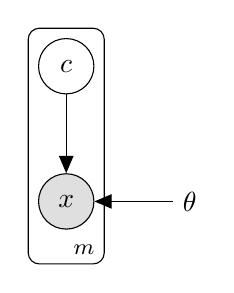
\begin{tikzpicture}
    % Define nodes
    \node[latent]		(z)		{$ c $};
    \node[obs, below = of z]		(x)		{$ x $};
    \node[right = of x]		(theta)		{$ \theta $};
    
    
    % Connect nodes
    \edge{z,theta}{x};
    
    % add plates
    \plate {x-sentence} {(x)(z)} {$ m $};
    \end{tikzpicture}
    \end{column}
    \begin{column}{0.7\textwidth}
    	\begin{itemize}\pause
			\item sample a latent class $c \in \{1, \ldots, K\}$ \\ 
			$c \sim \mathcal \mathcal U(\frac{1}{K})$ \pause
			\item generate categorical observation $x$ from $c$ \\
			$x \sim P(X|C=c)$  \pause
			\item where $P(X|C=c) = \Cat(f_\theta(c))$  \pause
			\begin{itemize}
				\item e.g. $f_\theta(c) = \softmax(W^{(f)} g(c) + b^{(f)})$ \\ \pause
				and $g(c) = \tanh(W^{(g)} r(c) + b^{(g)})$ \\ \pause
				and $r(c) = E c$ \pause				
			\end{itemize}
			\item with $\theta=(E, W^{(f)},  b^{(f)},  W^{(g)},  b^{(g)})$
		\end{itemize}
    \end{column}
    \end{columns}
    \pause
    
    $$P(x) = \underbrace{\sum_{c=1}^K \underbrace{P(c) P(x|c)}_{\textcolor{blue}{\text{differentiable function of }\theta}}}_{\alert{\text{tractable for small }K}}$$

	\pause
	Gradient-based optimisation! $\nabla_\theta \log P_\theta(x)$
}




\frame{
	\frametitle{Generative models with neural networks}
	
	Continuous mixture model
	
	\begin{columns}
	\begin{column}{0.2\textwidth}
	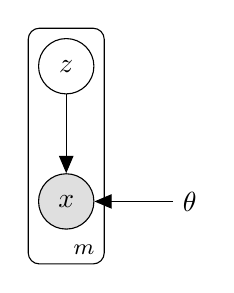
\begin{tikzpicture}
    % Define nodes
    \node[latent]		(z)		{$ z $};
    \node[obs, below = of z]		(x)		{$ x $};
    \node[right = of x]		(theta)		{$ \theta $};
    
    
    % Connect nodes
    \edge{z,theta}{x};
    
    % add plates
    \plate {x-sentence} {(x)(z)} {$ m $};
    \end{tikzpicture}
    \end{column}
    \begin{column}{0.7\textwidth}
    	\begin{itemize}\pause
			\item sample a latent embedding $z \in \mathbb R^d$ \\ 
			$z \sim \mathcal N(0, I)$ \pause
			\item generate categorical observation $x$ from $z$ \\
			$x \sim P(X|Z=z)$  \pause
			\item where $P(X|Z=z) = \Cat(f_\theta(z))$  \pause
			\begin{itemize}
				\item e.g. $f_\theta(z) = \softmax(W^{(f)} g(z) + b^{(f)})$ \\ \pause
				and $g(z) = \tanh(W^{(g)} z + b^{(g)})$ \\
			\end{itemize}\pause
			\item with $\theta=(W^{(f)},  b^{(f)},  W^{(g)},  b^{(g)})$ \pause
			\item \alert{Intractability} \pause
			\begin{itemize}
				\item $P(x) = \int p(z) P(x|z) \mathrm{d}z$
				\item $P(z|x) = \frac{p(z)P(x|z)}{\int p(z') P(x|z') \mathrm{d}z'}$
			\end{itemize}
		\end{itemize}
    \end{column}
    \end{columns}

	
}


\frame{
	\frametitle{Variational inference}
	
	but we know VI :D  \pause 
	
	\begin{columns}
	\begin{column}{0.2\textwidth}
	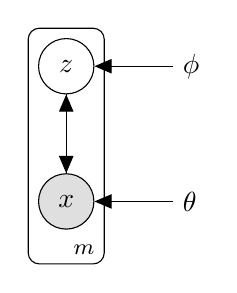
\begin{tikzpicture}
    % Define nodes
    \node[latent]		(z)		{$ z $};
    \node[obs, below = of z]		(x)		{$ x $};
    \node[right = of x]		(theta)		{$ \theta $};
    \node[right = of z]		(phi)		{$ \phi $};
    
    % Connect nodes
    \edge{z,theta}{x};
    \edge[dashed, bend right]{x}{z};
    \edge{phi}{z};
    
    % add plates
    \plate {x-sentence} {(x)(z)} {$ m $};
    \end{tikzpicture}
    \end{column}
    \begin{column}{0.7\textwidth}
    	\begin{itemize}
			\item approximate the posterior with \\ 
			$q_\phi(Z|x) = \mathcal N(\mu_\phi(x), I \sigma^2_\phi(x))$ \pause
			\item where 
			\begin{itemize}
				\item $\mu_\phi(x) = W^{(\mu)} u(x) + b^{(\mu)}$ \\
				e.g. $u(x) = \tanh(W^{(u)} r(x) + b^{(u)})$\\
				and  $r(x) = E^{(u)} x$  \pause
				\item $\sigma_\phi(x) = W^{(\sigma)} v(x) + b^{(\sigma)}$ \\
				e.g. $v(x) = \tanh(W^{(v)} r(x) + b^{(v)})$ \\
				and  $r(x) = E^{(v)} x$ \pause
			\end{itemize}
			\item with $\phi=(E^{(u,v)}, W^{(u,v,\mu,\sigma)}, b^{(u,v,\mu,\sigma)})$		\pause	
		\end{itemize}
    \end{column}
    \end{columns}
    
    Mean field assumption
	\begin{itemize}
		\item $q_{\phi_i}(Z|x_i)$ is specified for each observation $x_i$ by locally predicting its mean and variance
	\end{itemize}
}

\frame{
	\frametitle{Approximate inference by optimisation}
	
	 Maximise ELBO
    $$\log P_\theta(x) \ge \underbrace{\mathbb E_{q_\phi(Z|x)}\left[\log \frac{p_\theta(Z)}{q_\phi(Z|x)}\right]}_{\textcolor{blue}{-\KL(q_\theta(Z|x)||p_\theta(Z))}} + \underbrace{\mathbb E_{q_\phi(Z|x)}\left[\log P_\theta(X=x|Z) \right]}_{\alert{\text{intractable!}}}$$

	~\pause
	
	Prior term
	$$\KL(q_\phi(Z|x)||p_\theta(Z)) = - \frac{1}{2} \sum_{j=1}^d (1 + \log \sigma^2_\phi(x)_j - \mu_\phi^2(x)_j - \sigma^2_\phi(x)_j)$$
	
	\pause
	Likelihood term is intractable
	\begin{itemize}
		\item the Categorical likelihood is not conjugate with the Normal approximate posterior
	\end{itemize}

}

\frame{
	\frametitle{Change of variable for location-scale distributions}
	
	For $Z \sim \mathcal N(\mu, \sigma^2)$ we can re-express $Z$ in terms of $E \sim \mathcal N(0,1)$
	\begin{itemize}
		\item $Z = \mu + \sigma E$
	\end{itemize} \pause
	then we can re-express expectations
	$$\mathbb E_{\mathcal N(\mu, \sigma^2)}[f(Z)] = \mathbb E_{\mathcal N(0,I)}[f(\mu + \sigma E)]$$ \pause
	
	back to the ELBO
	$$\mathbb E_{q_\phi(Z|x)}\left[\log P(x|Z) \right] = \mathbb E_{\epsilon \sim N(0, I)}\left[\log P(x|Z=\mu_\phi(x) + \sigma_\phi(x) \epsilon)) \right]$$
}

\frame{
	\frametitle{Monte Carlo estimate}
	
	\begin{equation*}
	\begin{aligned}
		\mathbb E_{q_\phi(Z|x)}\left[\log P(x|Z) \right] &= \mathbb E_{\epsilon \sim N(0, I)}\left[\log P(x|Z=\mu_\phi(x) + \sigma_\phi(x) \epsilon)) \right] \\
		&\approx \frac{1}{N} \sum_{n=1}^N \log P\left(x|\mu_\phi(x) + \sigma_\phi(x) \epsilon^{(n)}\right)
	\end{aligned}
	\end{equation*}
}

\frame{
	\frametitle{MC estimate of the ELBO}
	
	\begin{equation*}
	\begin{aligned}
	\log P_\theta(x) &\ge \underbrace{\mathbb E_{q_\phi(Z|x)}\left[\log \frac{p_\theta(Z)}{q_\phi(Z|x)}\right]}_{\textcolor{blue}{-\KL(q_\theta(Z|x)||p_\theta(Z))}} + \underbrace{\mathbb E_{q_\phi(Z|x)}\left[\log P_\theta(X=x|Z) \right]}_{\alert{\text{intractable!}}}\\
	&\approx \underbrace{\frac{1}{2} \sum_{j=1}^d \left(1 + \log \sigma^2_\phi(x)_j - \mu_\phi^2(x)_j - \sigma^2_\phi(x)_j\right)}_{\textcolor{blue}{-\KL(q_\theta(Z|x)||p_\theta(Z))}} \\
	&\quad + \underbrace{\log P_\theta\left(x|\mu_\phi(x) + \sigma_\phi(x) \epsilon \right)}_{\textcolor{blue}{\text{single-sample estimate}}}
	\end{aligned}
	\end{equation*}

}

\frame{
	\frametitle{Gradient-based optimisation}
	
	Let $\mathcal L(\theta, \phi|x)$ be our objective function\\
	\begin{equation*}
	\begin{aligned}
	\mathcal L(\theta, \phi|x) &= \underbrace{ \frac{1}{2} \sum_{j=1}^d \left(1 + \log \sigma^2_\phi(x)_j - \mu_\phi^2(x)_j - \sigma^2_\phi(x)_j\right)}_{\textcolor{blue}{\text{differentiable function of }\phi}} \\
	&\quad + \underbrace{\log P_\theta\left(x|\mu_\phi(x) + \sigma_\phi(x) \epsilon \right)}_{\textcolor{blue}{\text{differentiable function of }\theta\text{ and }\phi}}
	\end{aligned}
	\end{equation*} \pause
	
	~
	
	We can update $\theta$ and $\phi$ using stochastic gradient steps
	\begin{itemize}
		\item we know chain rule (thus we can get a gradient)
		\item we have a noisy though unbiased estimate
		\item guaranteed convergence to a local optimum of $\mathcal L$\\
		(with appropriate learning rate schedule)
	\end{itemize}
}

\frame{
	\frametitle{Further reading}
	
	\begin{itemize}
		\item Auto-Encoding variational Bayes \citep{Kingma+2014:VAE}
	\end{itemize}
}

%\include{applications}

\begin{frame}{Summary}

Deep learning in NLP
\begin{itemize}
	\item task-driven feature extraction
	\item models with more realistic assumptions
\end{itemize}

~

Probabilistic modelling 
\begin{itemize}
	\item better (or at least more explicit) statistical assumptions
	\item compact models
	\item semi-supervised learning
\end{itemize}


\end{frame}

\begin{frame}[allowframebreaks]{Literature}
\bibliographystyle{plainnat}
\small
\bibliography{VI}
%\nocite{KingmaWelling:2013}
%\nocite{HintonEtAl:1995}
%\nocite{RezendeEtAl:2014}
%\nocite{TitsiasLazarogredilla:2014}
%\nocite{BergkirkpatrickEtAl:2010}
%\nocite{KucukelbirEtAl:2017}
\end{frame}



\end{document}
\grid